\documentclass[a4paper]{article}

%% Language and font encodings
\usepackage[portuges]{babel}
\usepackage{fontspec}

%% Sets page size and margins
\usepackage[a4paper,top=3cm,bottom=2cm,left=3cm,right=3cm,marginparwidth=1.75cm]{geometry}

%% Useful packages
\usepackage{amsmath,amsthm,amssymb,amsfonts}
\usepackage{graphicx}
\usepackage[colorinlistoftodos]{todonotes}
\usepackage[colorlinks=true, allcolors=blue]{hyperref}

\newcommand{\R}{\mathbb{R}}
\newcommand{\N}{\mathbb{N}}
\newcommand{\Z}{\mathbb{Z}}
\providecommand{\C}{\mathbb{C}}

\theoremstyle{definition}
\newtheorem{defin}{Definição}

\theoremstyle{plain}
\newtheorem{theorem}[defin]{Teorema}
\newtheorem{corollary}[defin]{Corolário}



\title{Project 1}

\author{Allen Zhang\\
        Joseph Hawkins\\
        Anthony de Rose \\
}

\date{7/13/2020}

\begin{document}
\maketitle


\section*{Part 0 Setup your Environment [10 points]}
We used grid-world-generator.py with some modifications to create 50 mazes using recursive dfs. We also initialized a random start and random goal node as well. The color scheme makes it a bit difficult to distinguish between unblocked and block nodes, but the final solution contains a much cleaner and more identifiable color scheme: black squares are blocked squares, white squares are unblocked squares, blue is the start, orange is the goal, and yellow is the path followed. Here is a closeup of a finished maze.\\
\begin{center}
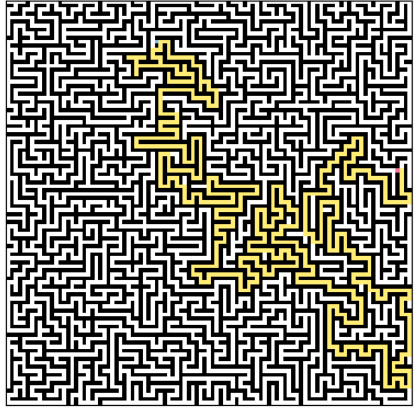
\includegraphics[scale= .7]{part0.PNG}
\end{center}

\section*{Part 1 Understanding the methods [10 points]}

a) Explain in your report why the first move of the agent for the example search problem from Figure 8 is to the east rather than the north given that the agent does not know initially which cells are blocked.
\begin{center}
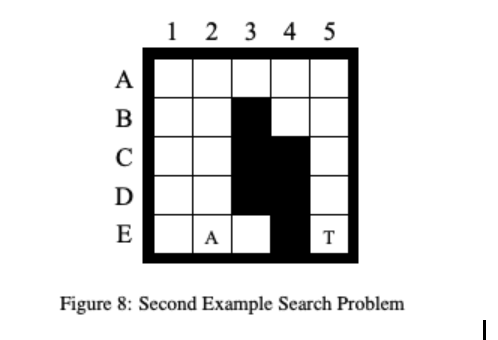
\includegraphics{part1 problem.PNG}
\end{center}
The states that we can visit from A are D2, E1, and E3. The f values are the sum of the g value and h-value. The g-values are 1 for all of the nodes. The h-value is the Manhattan distance to the goal state, and the agent assumes that all cells beyond its vision are not blocked. The h-value for the D2, E1, and E3 are 4, and 4, and 2. The f-value for E3 is 3, which is the smallest value, so we visit that state first.\\ b) This project argues that the agent is guaranteed to reach the target if it is not separated from it by blocked cells. Give a convincing argument that the agent in a finite gridworld indeed either reaches the target or discovers that this is impossible in finite time. Prove that the number of moves of the agent until it reaches the target or discovers that this is impossible is bounded from above by the number of unblocked cells squared. 
\\ \\ 
In a finite gridworld, there will only be a finite number of cells. Each cell has neighboring cells, therefore, assuming there are no blocked cells, we can go from any cell in the gridworld to any other cell by following neighborings. If there are blocked cells, we can also go from an unblocked cell to another unblocked cell as long as a blocked cell or the border region of the gridworld does not block the path. \\
Because A* has a closed list which keeps all already expanded cells, it will never expand to those cells again. This allows A* to follow the neighbors to find a path from a start to a goal if there is no blockage between both nodes. Otherwise, the algorithm will say that no path can be found. To continue, the repeated version of A* will execute A* multiple times finding either a path or saying there is no solution. The worst possible case that can happen is every single cell of the gridworld is discovered in finding a path. Everytime we hit a blockage, A* will run again in repeated A*. This can be summarized as a loop that cycles through computing the path and moving the agent. \\
Also, notice how there can only be at most x cells in a gridworld. Say that m is the number of moves an agent makes. So, moves will always be less than the total number of cells. m <= x\\
Lets also call i the number of iterations of the loop that happens in repeated forward A*. Due to the nature of A*, the number of iterations will always be less than or equal to the number of cells. Therefore, i <= x\\
Combining our past discoveries:\\
m <= x and i <= x \\
As a reminder, x is the number of unblocked cells, i is the number of loop iterations, m is the number of moves an agent makes in a loop, and m*i is presumably the total number of agent moves.\\
$m*i <= x^2$\\
The number of moves the agent makes until it reaches the goal or discovers there isn’t a solution is capped by the number of unblocked cells squared. 



\section*{Part 2 - The Effects of Ties [15 points]}
Repeated Forward A* needs to break ties to decide which cell to expand next if several cells have the same smallest f-value. It can either break ties in favor of cells with smaller g-values or in favor of cells with larger g-values. Implement and compare both versions of Repeated Forward A* with respect to their runtime or, equivalently, number of expanded cells. Explain your observations in detail, that is, explain what you observed and give a reason for the observation. \\We implemented a Repeated Forward A* algorithm with tie-breakers that favor either smaller g-values or larger g-values. This is done by changing how we sort nodes into the heap. We implemented our own comparator for comparing two nodes by looking at their f-values. Inside this comparator, nodes with the same f-value and larger g-value would  be considered smaller for large g, and nodes with the same f-value and smaller g-value would be considered smaller for small g. \\ Large g was significantly faster than small g. On average, large g expanded 343,958 nodes while small g expanded 733,771 nodes for each maze. The graph below shows the number of expansions for each maze. 
\begin{center}
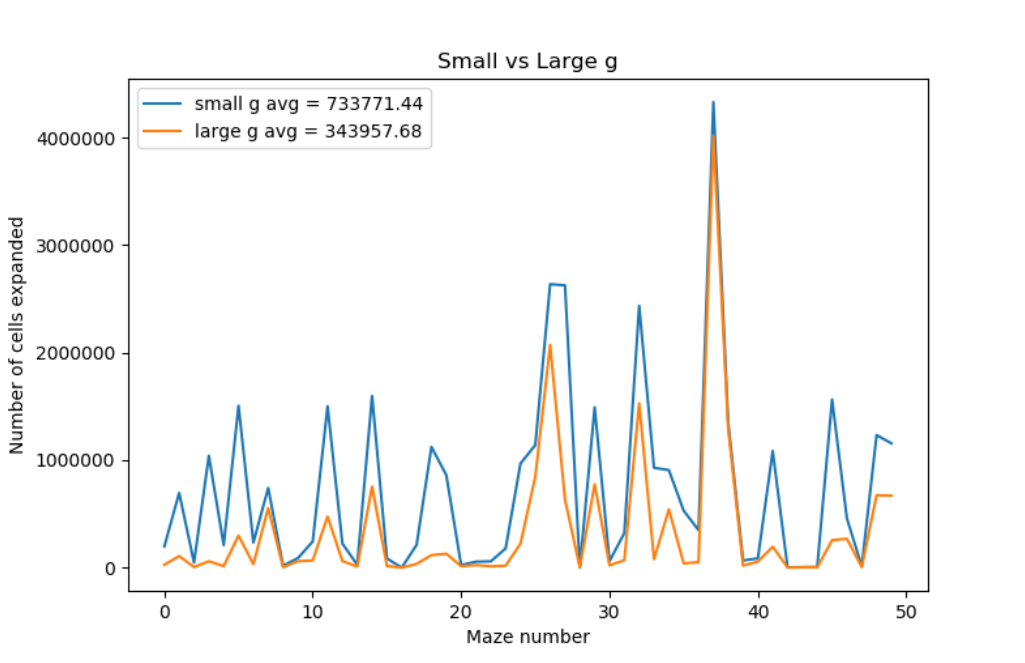
\includegraphics[scale=.7]{part2graph.PNG}
\end{center}
This also confirms the theoretical explanation as well. Large-g A* acts almost like DFS search, in that it moves along a path towards the goal. Small-g A* acts like a BFS search, expanding all the neighboring nodes at a single level before moving to the next level. For a maze search, the small-g tie breaker is very inefficient, since it will expand many unnecessary nodes. In a larger maze, this can become even more pronounced. 
\begin{center}
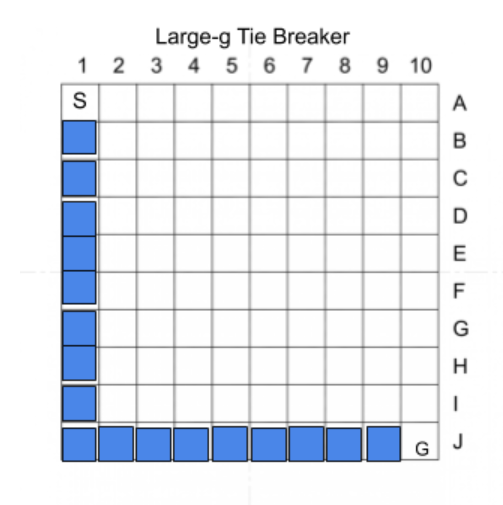
\includegraphics[scale=.6]{part2large.PNG}
\end{center}

\begin{center}
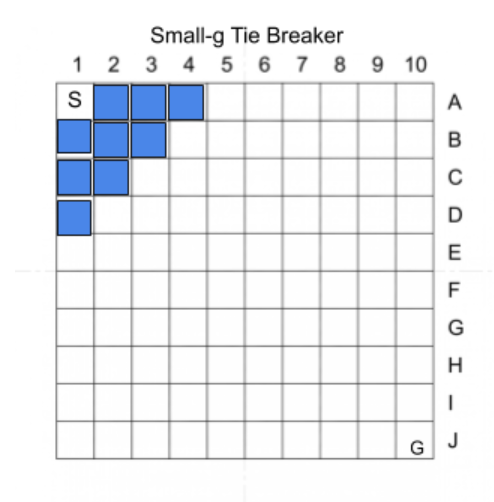
\includegraphics[scale=.6]{part2small.PNG}
\end{center}

This is the worst case, but the small-g as seen here would expand nearly every cell before reaching G, which is very inefficient.

\section*{Part 3 - Forward vs. Backward [20 points]}
Repeated Forward A* was significantly faster than Repeated Backward A*. Forward A* on average expanded 343,958 nodes while backwards A* expanded 2,303,843 nodes. This makes sense, since backward A* starts at the goal and plans the path towards the start. Therefore, it can expand a lot of unnecessary nodes. Imagine there are a few blocked cells near the starting node, and start and goal are relatively far apart. With backwards A*, we would find a path all the way until we reach a blocked node. However, now the f value of the node’s neighbors might increase by at least one, since now we need to move around the cell instead of through it. The g value increases by at least one but the h value may not decrease by the same amount, since the Manhattan distance may not actually. As a result, we must expand a node that is close to the goal and go all the way to start again, since those nodes all have smaller f values. \\
\begin{center}
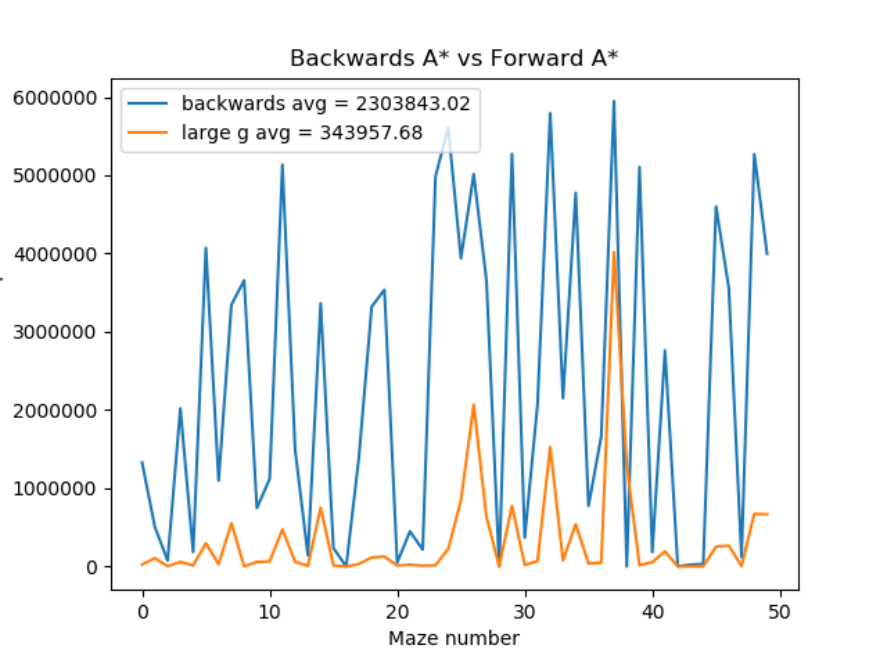
\includegraphics[scale=.6]{backvsforw.PNG}
\end{center}
In the case of forward A*, once we reach a blocked node, it is also true we also need to start expanding smaller f value nodes as well. However, since the start is very close to the known blocked nodes, we do not need to expand a ton of nodes before reaching the blocked nodes again. Backwards A* on the other hand, must expand many nodes until it reaches the known blocked nodes, which is very inefficient.\\
\begin{center}
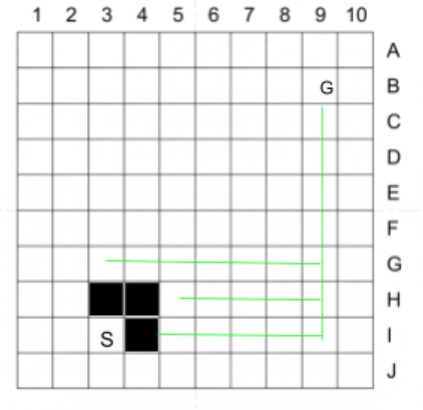
\includegraphics[scale=.6]{part3.PNG}
\end{center}

If we look at the example above, all nodes in green have an f-value of 13 for backwards A*. If we want to go around those blocked nodes, the f-value increases. J5 would have an f-val of 15, so it would need to wait for all nodes with smaller f-values to get expanded first. Backwards A* is inefficient since it must expand all of these nodes before moving around blocked nodes. If we started at S instead, we would see that the nodes are blocked and start expanding other nodes much sooner, since we have to travel much less to reach blocked nodes.

\section*{Part 4 - Heuristics in the Adaptive A* [20 points]}
Because the agent can only move in four directions, Manhattan Distance is what allows our agent to move vertically in a sense. The agent will move vertically until it is on the same level horizontally as the goal and then proceed to move horizontally towards the goal. This assumes there are no blocked cells. If there are blocked cells, then the agent will have to make detours which will increase the cost. Not using Manhattan Distance will cause our agent to move not efficiently. To prove that Manhattan Distance is a consistent heuristic let's assume the opposite.\\For sake of contradiction assume manhattan distance is an inconsistent heuristic:\\
    $\exists$(a, c, b) : h(a) >= c(a, c, b) + h(b)\\
Where c(a, c, b) is the cost of going from a node, a, to another node, b, using action cost, c. \\
Moving h(y) to the other side of the equation: \\
    $\exists$(a, c, b): h(a) - h(b) >= c(a, c, b) \\
h(a) and h(b) is the Manhattan distance from node a or node b to the goal node, therefore:\\
	h(a=>b) : |h(a) - h(b)|\\
h(a=>b) is the Manhattan Distance from a to b. \\
If we combine what we know:\\
	$\exists$(a, c, b) : h(a=>b) >= c(a, c, b)\\
Knowing Manhattan Distance is just the difference between two nodes or points on a 2d grid:\\
	h(a=>b) = | x(a) - x(b) | + | y(a) - y(b) |\\
The only case for this equation h(a=>b) to fail is when both points are equal. This makes h(a=>b) = 0. Thus, allowing a case to be inconsistent. Since the agent is living in a gridworld, this will never be the case due to the up, down, left, right action nature and we will never compare two nodes at the same location. The only case that allows this to be inconsistent is when both nodes are the same, which is trivial. Therefore, Manhattan distances must be consistent in gridworlds. 
\\ \\
Furthermore, it is argued that “The h-values h-new(s) ... are not only admissible but also consistent.” Prove that Adaptive A* leaves initially consistent h-values consistent even if action costs can increase. \\\\
Let function g(goal) be the smallest goal cost by A*at the current moment of gridworld knowledge. Let g(a) be the smallest goal cost by A* at the current moment of gridworld knowledge to a. Therefore, g(goal) - g(a) is the smallest cost from a to goal under current knowledge of the gridworld. As we gain more knowledge of the gridworld and explore, we increase the number of unblocked cells. So, the cost to get to the goal will only increase. The heuristic used by adaptive A* is the smallest cost from a to goal having the current knowledge at any given time. Using a direct proof let us prove this. \\
Let h(x) be the new heuristic used by adaptive A* from x to goal. So, we can see it as:\\
	h(x) = g(goal) - g(x)\\
Let’s assume h(x) is a consistent heuristic: \\
	$\forall$(a,c,b) : h(a) <= c(a,c,b) + h(b)\\
Knowing that h(x) = g(goal) - g(x):\\
    $\forall$(a,c,b) : h(a) <= c(a,c,b) + g(goal) - g(b)\\
Simplifying:\\
    $\forall$(a,c,b) : g(b) - g(a) <= c(a,c,b)\\
c(a,c,b) is smallest if a and b are on the same level and no cells between them are blocked. In this case, the difference between them is just the distance between a and b. Assuming we get g(a) and g(b) from A* with Manhattan distance which is a consistent heuristic. Sp g(a) and g(b) are the smallest in cost from the start to a and b, Therefore, g(b) - g(a) is the difference in either cost or distance between b and a. \\
	g(b) - g(a) = c(a,c,b)\\
Taking the smallest c(a,c,b) we prove:\\
	 $\forall$(a,c,b) : g(b) - g(a) <= c(a,c,b) is true. \\
Therefore, the new heuristics used by adaptive A* are consistent. \\

\section*{Part 5 - Heuristics in the Adaptive A* [15 points]}
We found that Adaptive A* is slightly faster than Repeated Forward A*. Adaptive A* updates h values of the expanded cells to a bigger heuristic, which is more accurate after each time the program runs computePath() since it accounts for blocked nodes. Therefore, better choices can be made by Adaptive A* regarding the cells in the open list than Repeated Forward A* since we provide a more accurate heuristic. Thus, the number of cells expanded after each Adaptive A* will be fewer than Repeated Forward A*. Also, everytime there is a detour near the current position of Adaptive A*, the cells near it will have their h value changed. However, Adaptive A* doesn’t generally search back to cells it already moved to so these changes in h values near detours didn’t do much. There is some time spent traversing the closed list and changing heuristics after each pass of Adaptive A*, but overall runtime for Adaptive A* was still much better because we needed to expanded significantly fewer nodes. The average number of nodes expanded for Adaptive A* was 111,277 while Repeated Forward A* was 343,958.

\begin{center}
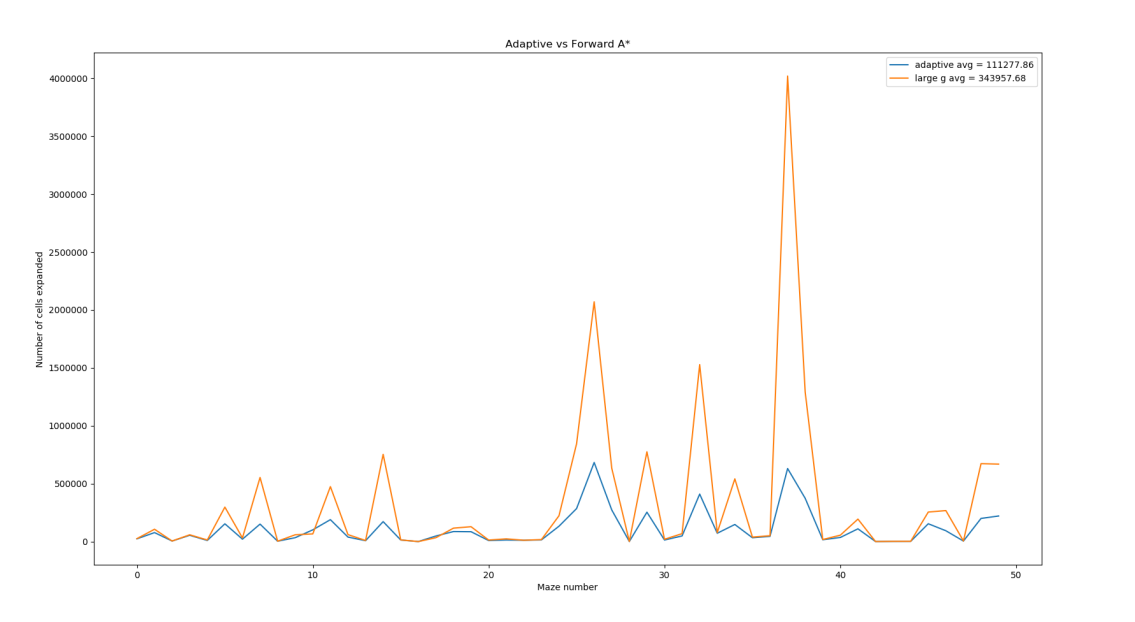
\includegraphics[scale=.8]{part5.PNG}
\end{center}



\section*{Part 6 - Memory Issues [10 points]}

Additional ways to reduce the memory consumption:\\
We are storing a number of variables that we don’t necessarily have to. For example, the x and y values of a node can be converted into a single int. We do not need to store other variables such as the f and h values, we could calculate them when needed. We are also using a variable called alg in the Node class which is a boolean variable determining whether to use small or large g. We could have implemented this differently, by checking the type of tie breaker with an if statement every time we do a comparison. \\
The tree pointer can be smaller; it can be two bits. Each combination of the two bits can represent the direction of the parent. Since we know the parent must be next to the child node, we only need 4 to represent the parent. We can calculate the parent easily by adding or subtracting one to the row or col depending on the bits.\\
Calculating the amount of memory for gridworlds of size 1001x1001:\\
A cell has a 7 int values, 1 character, 1 pointers to other nodes\\
7* 4 + 1 + 4 = 33\\
In a gridworld of 1001 x 1001: 1001 * 1001 * 33 = 33,066,033 bytes = 33 MB\\
Largest gridworld that can operate within 4 megabytes: \\
Every cell is 41 bytes: (4 *1024*1024)/ 33 = 127100.12 cells = 356x356\\


\end{document}